\documentclass{article}

\usepackage{amsmath}
\usepackage{graphicx}

\newcommand{\rr}{\mathbf{r}}

\begin{document}

{\bf Quiz \#12; Tuesday, date: 04/17/2018}

{\bf MATH 53 Multivariable Calculus with Stankova}

{\bf Section \#114; time: 2 -- 3:30 pm}

{\bf GSI name: Kenneth Hung}

{\bf Student name: SOLUTIONS}

\vspace*{0.25in}

\begin{enumerate}
\item Use Green's Theorem to evaluate the line integral along the given positively oriented curve.
\[
\int_C \frac{1}{4} y^4 x \,dx + \frac{5}{2}y^3 x^2 \,dy,
\]
where $C$ is the ellipse $x^2 + y^2 = 4$.

{\em Solution.} By Green's Theorem,
\[
\int_C \frac{1}{4} y^4 x \,dx + \frac{5}{2}y^3 x^2 \,dy = \int_D \left(5y^3 x - y^3 x\right) \,dA = \int_D 4y^3 x \,dA,
\]
where $D$ is the disc $\{x^2 + y^2 \le 4\}$. This disc can be reparametrized by $x = r \cos \theta$ and $y = r \sin \theta$ where $0 \le r \le 1$ and $0 \le \theta \le 2\pi$. The Jacobian is then
\[
\begin{vmatrix}
\cos \theta & -r \sin \theta \\
\sin \theta & r \cos \theta
\end{vmatrix} = r,
\]
so the integral is
\begin{align*}
\int_D 4y^3x \,dA & = \int_0^{2\pi} \int_0^2 4 (r \sin \theta)^3 (r \cos \theta) r \,dr \,d\theta \\
& = \left(\int_0^{2\pi} 4 \sin^3 \theta \cos \theta \,d\theta\right) \left(\int_0^2 r^5 \,dr\right) \\
& = \left[\sin^4 \theta\right]_0^{2\pi} \left[\frac{1}{6} r^6\right]_0^2 \\
& = 0.
\end{align*}

\item {\em True / False?} Fix two points $A$ and $B$ in a simply connected domain $D$. If $\int_C \mathbf{F} \cdot d\rr$ is the same for all paths $C$ from $A$ to $B$, then $\mathbf{F}$ must be conservative on $D$.

{\em Solution.} {\bf True.} For any two paths $C_1$ and $C_2$ that shares the same initial point $A'$ and terminal point $B'$, we can do the following: Pick a path $C_A$ from $A$ to $A'$ and a path $C_B$ from $B$ to $B'$. So $C_A \cup C_1 \cup C_B$ and $C_A \cup C_2 \cup C_B$ are both paths from $A$ and $B$. Hence the integral $\int_{C_A \cup C_1 \cup C_B} \mathbf{F} \cdot d\rr$ and $\int_{C_A \cup C_2 \cup C_B} \mathbf{F} \cdot d\rr$ must be the same. Since
\[
\int_{C_A \cup C_1 \cup C_B} \mathbf{F} \cdot d\rr = \int_{C_A} \mathbf{F} \cdot d\rr + \int_{C_1} \mathbf{F} \cdot d\rr + \int_{C_1} \mathbf{F} \cdot d\rr
\]
and the same for $\int_{C_A \cup C_2 \cup C_B} \mathbf{F} \cdot d\rr$, we have
\[
\int_{C_1} \mathbf{F} \cdot d\rr = \int_{C_2} \mathbf{F} \cdot d\rr,
\]
and so the integral is path independent on $D$. The result follows from Theorem 4.

\item {\em True / False?} Suppose $P$ and $Q$ has continuous partial derivatives everywhere. Green's Theorem cannot help us in computing line integral $\int_C \mathbf{F} \cdot d\rr$ where $C$ is given below.
\begin{center}
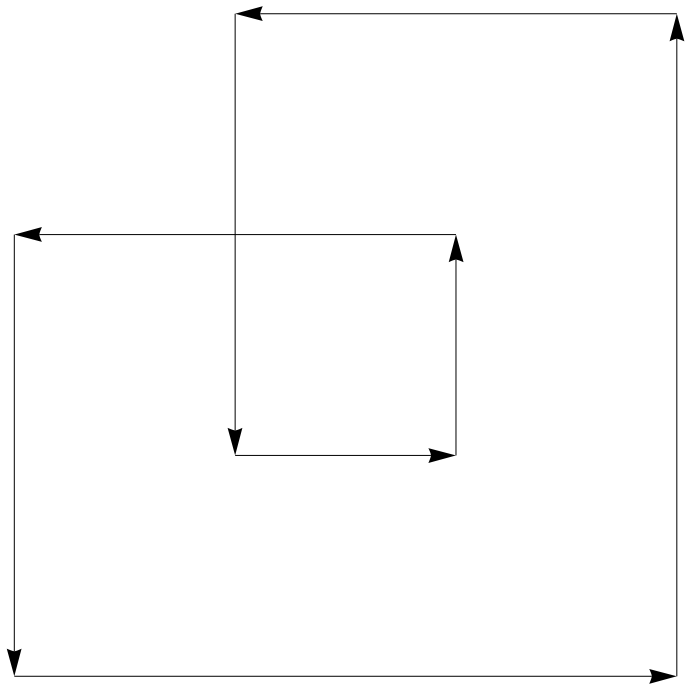
\includegraphics[width=0.33\textwidth]{quiz12dis114pic}
\end{center}

{\em Solution.} {\bf False.} The integral can be broken down into the line integral along the outside boundary (counterclockwise) and along the inside boundary (clockwise), so we can still apply Green's Theorem even when this is not a simple closed curve.
\end{enumerate}

\end{document}